\section{Experimentación}

\subsection{Metodología}

Los siguientes experimentos fueron generados a partir de archivos de entrada para nuestro algoritmo que siguen ciertas reglas. En todos los casos donde analizamos el tiempo de ejecución de los algoritmos, decidimos generar 100 instancias para el mismo experimento y luego tomar la media. Esto se debe a que el uso del CPU no es uniforme y lleva a que las mediciones estén sesgadas, principalmente causado por el algoritmo de scheduling del SO y el uso de memoria.

\subsection{Evaluación de los métodos}

\subsubsection{Variando la dimensión}

Para este experimento, decidimos analizar el tiempo de ejecución de nuestro algoritmo en función de la dimension de la matriz $A$. A priori, dado que ambos algoritmos son \order{n^3} y solo se están ejecutando sobre una única instancia, esperamos que los tiempos de ejecución sean sumamente similares.

Para la generación de instancias, utilizamos $m = 3$, $n = 3$, $r_i = 10$, $r_e = 100$, $ninst = 1$, $m = 10$ y $n$ aumentando de a 1. Aumentamos solo $n$ para aumentar la dimension de la matriz A dado que lo que relevante al tiempo de ejecución final del algoritmo es la dimension total, no de donde proviene la misma.

\begin{figure}[h]
\centering
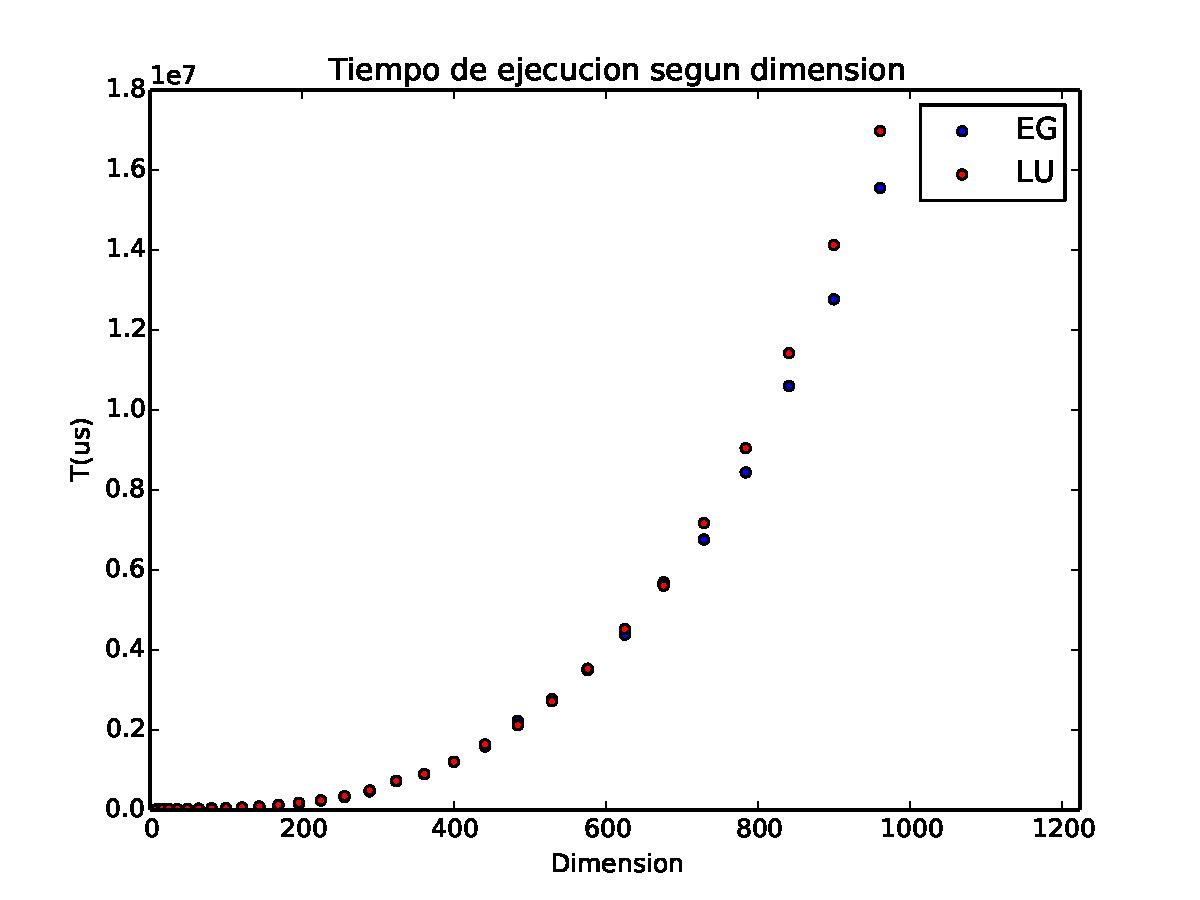
\includegraphics[scale=0.7]{graficos/dimVariable.pdf}
\caption{Tiempos de ejecución según dimension, EG vs LU.}
\end{figure}

Como se puede observar en estos gráficos, ambos algoritmos tienen casi los mismos tiempos de ejecución para una dimension dada. Esto coincide con la teoría.

\pagebreak

\subsubsection{Variando numero de instancias}

Para este experimento la idea es ver la diferencia en performance de la eliminación gausiana y la factorización LU a medida que aumenta el numero de instancias, es decir, a medida que cambiamos la matriz $b$. Aunque ambos algoritmos pertenecen a \order{n^3}, esperamos que la factorización LU sea superior a la eliminación gausiana dado que para la factorización LU el costo adicional de resolver otras instancias es de \order{n^2} (es un simple producto de matrices) mientras que la eliminación gausiana debe repetir todo el procedimiento en \order{n^3}.

Para generar las instancias utilizadas en el gráfico, estos fueron los valores que utilizamos: $m = 15$, $n = 15$, $r_i = 10$, $r_e = 100$, $ninst = 1$, $ninst$ aumentando de a 1.

\begin{figure}[h]
\centering
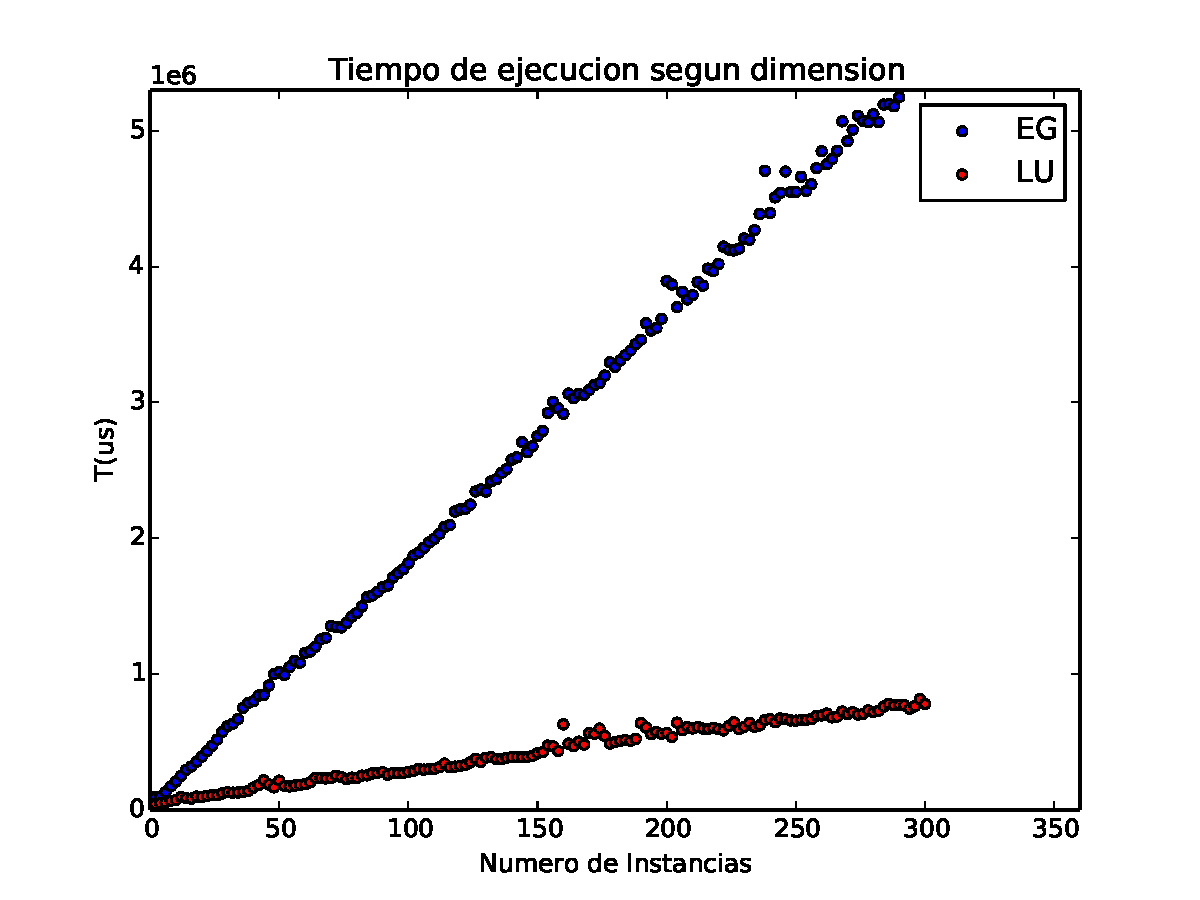
\includegraphics[scale=0.7]{graficos/ninstVariable.pdf}
\caption{Tiempos de ejecución variando numero de instancias, EG vs LU.}
\end{figure}

\textbf{Este testeo podríamos mejorarlo utilizando m y n mas chicos, como para tener mas datos y que se pueda ver la forma de la curva mejor.}

Coincidiendo nuevamente con la teoría, aquí es donde se pueden ver efectivamente las ganancias de la factorización LU. Aunque ambos algoritmos son cúbicos, en este problema la EG se ejecuta en \order{ninst \times n^3} mientras que la factorización LU en \order{n^3 + ninst \times n^2} $\in$ \order{n^3}. Esto se puede ver claramente en el gráfico.

\newpage
\subsection{Comportamiento del Sistema}

\subsection{Isoterma Empírica}

La idea de los siguientes experimentos es ver como varia la diferencia entre la isoterma empírica y la isoterma numérica a medida que cambiamos el nivel de granularidad, es decir, a medida que cambiamos la cantidad de radios y ángulos. Haremos este análisis para nuestros dos algoritmos de búsqueda.

\subsubsection*{Variando el numero de radios}

En este experimento vamos a evaluar la calidad de las isotermas a medida que aumentamos el numero de radios. A priori, esperábamos que la calidad de la solución fuese monótona creciente con el nivel de granularidad, en este caso particular en la cantidad de radios. A su vez, pensábamos que hacer un promedio pesado nos iba a acercar mas a la isoterma empírica que simplemente utilizando el método lower.

Para este experimento utilizamos instancias con los siguientes parámetros: $m = 8$, $n = 2$, $r_i = 10$, $r_e = 100$, $ninst = 1$, con $m$ aumentando de a 4. 

\begin{figure}[h]
  \centering
  \begin{minipage}[b]{0.49\textwidth}
    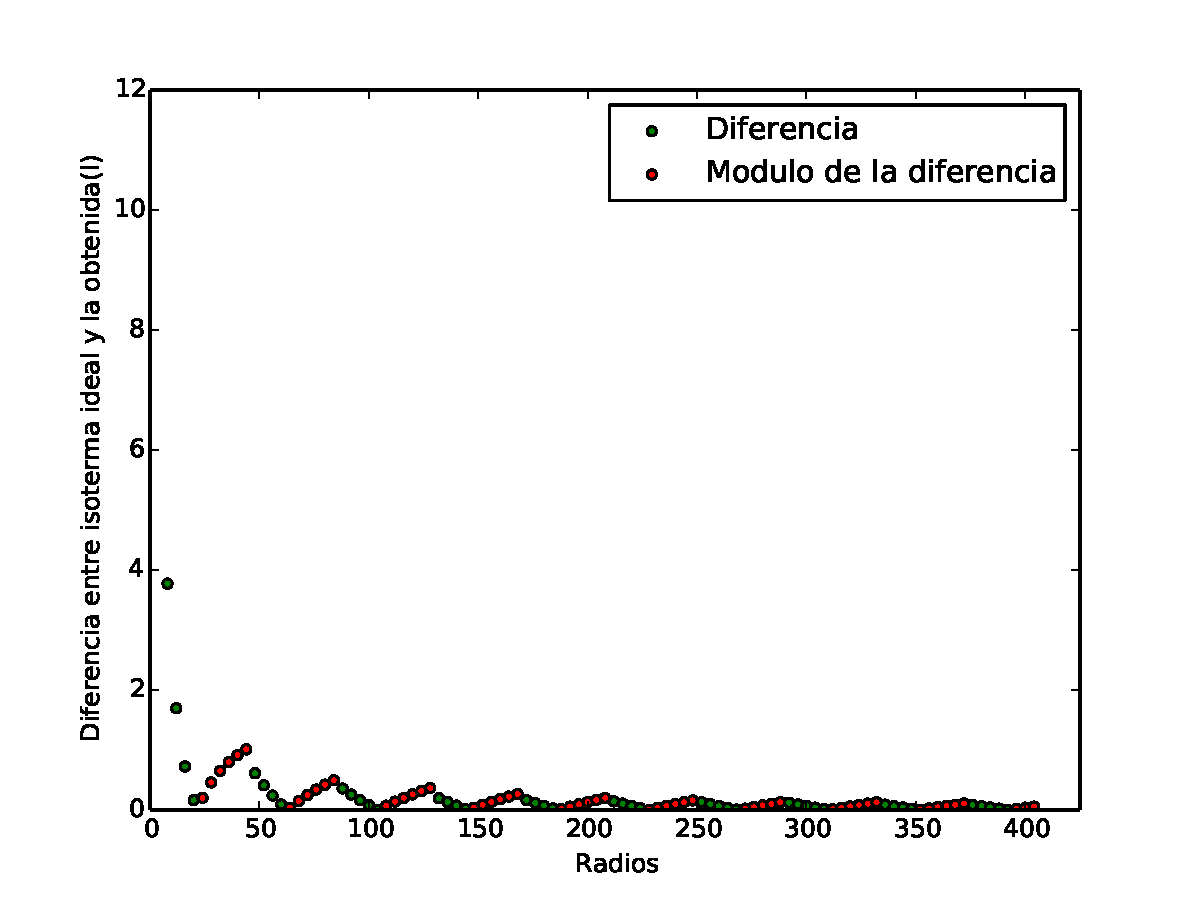
\includegraphics[width=\textwidth]{graficos/mVariable_l.pdf}
    \caption{Algoritmo: Lower}
  \end{minipage}
  \hfill
  \begin{minipage}[b]{0.49\textwidth}
    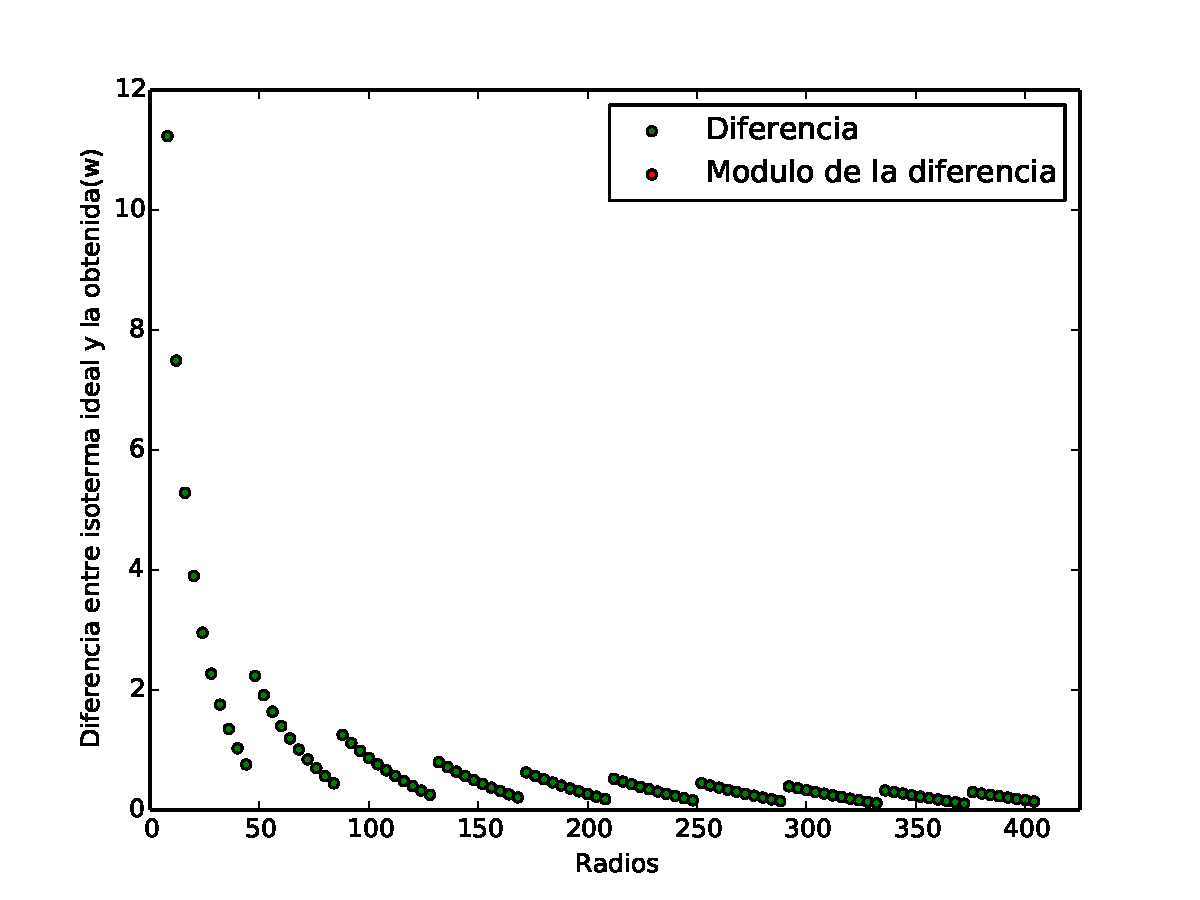
\includegraphics[width=\textwidth]{graficos/mVariable_w.pdf}
    \caption{Algoritmo: Weighted}
  \end{minipage}
\end{figure}

\textbf{Recordar analizar el trade off entre calidad de la solucion y tiempo de computo! Cambiarle escala al primer grafico?}

En contra de lo que pensábamos que iba a suceder, la calidad de la solución no es monótona creciente con el nivel de granularidad. A su vez, se puede ver que el algoritmo de tomar la isoterma justo menor al que se busca supera ampliamente al método weighted. En un principio pensábamos que nuestros experimentos podían estar mal, pero la realidad es que existe una explicación para estos resultados.

Cuando discretizamos el dominio de búsqueda en coordenadas polares y resolvemos el sistema lineal, lo que estamos haciendo es básicamente buscar una aproximación de la temperatura en cada punto de la discretización. Esta aproximación cambia a medida que variamos la granularidad. A mayor granularidad, la aproximación de la temperatura en cierto punto dado por cualquiera de nuestros algoritmos no es necesariamente mejor. La única forma de garantizar esto es que la nueva discretización no solo pase por los puntos que tenia la vieja discretización, si no que también agregue nuevos puntos. Dada la definición de nuestro problema, esto solo sucede cuando la granularidad en cualquiera de sus dimensiones aumenta en múltiplos de 2. Al observar estos múltiplos, aquí si podremos observar como la isoterma se comporta de la forma en la que nosotros originalmente habíamos esperado.

En cuanto a la razón de por que el metodo lower se comporta mejor que el weighted, conjeturamos que la razón mas significativa es el hecho de que quizás la temperatura no se propaga de forma uniforme en la pared del horno. El método weighted hace un promedio pesado asumiendo uniformidad, y quizá este supuesto es incorrecto.

\textbf{Hacer un testeo que muestre si el calor se propaga de forma uniforme. En clase te lo comente. Duplicas la temperatura externa, te fijas en cuanto se mueve la isoterma.}

\pagebreak

\subsubsection*{Variando el numero de ángulos}

Para este experimento, utilizaremos instancias con las siguientes características: $m = 20$, $n = 4$, $r_i = 10$, $r_e = 100$, $ninst = 1$, con $n$ aumentando de a 4.

A partir de las conclusiones del experimento anterior, ya no esperamos que la calidad de la solución mejore monotonamente a medida que aumentamos la cantidad de ángulos.

\begin{figure}[h]
  \centering
  \begin{minipage}[b]{0.49\textwidth}
    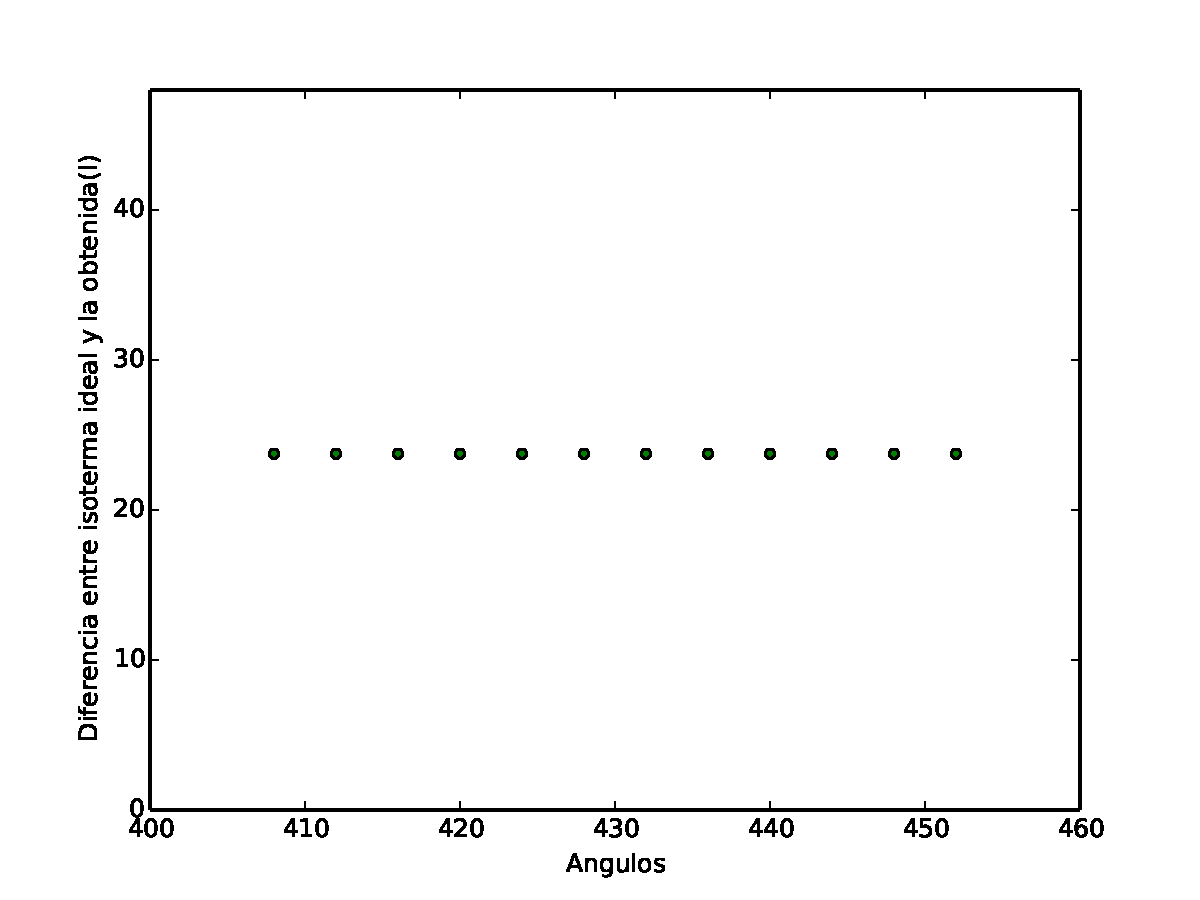
\includegraphics[width=\textwidth]{graficos/nVariable_l.pdf}
    \caption{Algoritmo: Lower}
  \end{minipage}
  \hfill
  \begin{minipage}[b]{0.49\textwidth}
    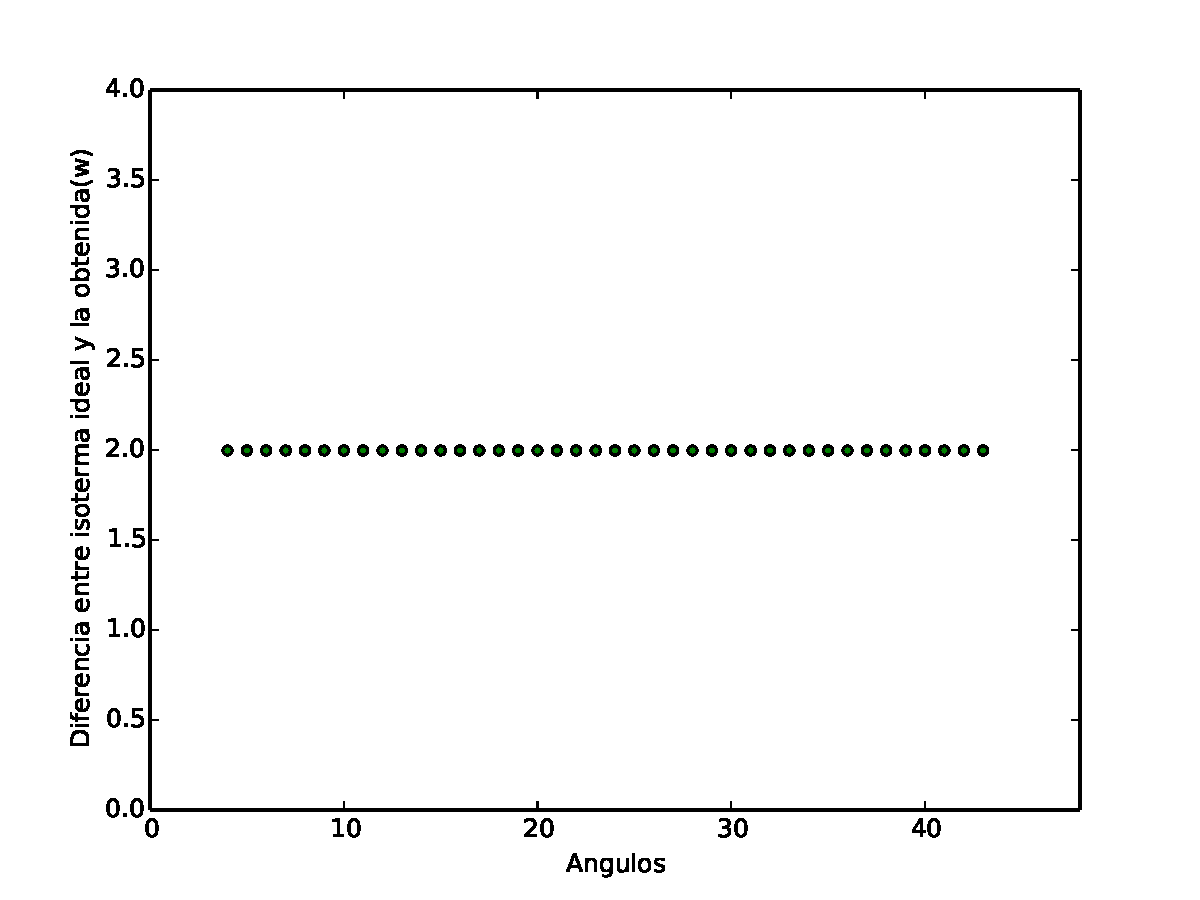
\includegraphics[width=\textwidth]{graficos/nVariable_w.pdf}
    \caption{Algoritmo: Weighted}
  \end{minipage}
\end{figure}

\textbf{Porque los ángulos arrancan en 400? Que escala fea che.}

Como se puede observar, ambos algoritmos tienen una performance sumamente similar y no se observan mejoras significativas en la calidad de las isotermas a medida que aumenta la cantidad de ángulos. Esto se debe a que nuestro caso de prueba fue un caso simétrico, donde para cualquier angulo las temperaturas para cualquier radio son idénticas. Esto nos trae una conclusión bastante importante: en casos que sean bastante simétricos, formar un caso simétrico tomando como temperatura externa el máximo, tomando solo 1 angulo y aumentando solo la cantidad de radios es la estrategia optima para evaluar la integridad estructural de un horno. Bajamos el tiempo de ejecución al no tener que evaluar todos los ángulos explotando la simetría del problema y solo aumentamos la dimension de granularidad relevante.

Variar el numero de ángulos cuando la temperatura es sumamente uniforme en el exterior puede tener efectos significativos sobre la calidad de la solución, aunque no tan significativos como la de variar los radios.

\textbf{Experimentar un poco con esta proposición?}

